\chapter{Introduction}
\label{c:introduction}
\IMRADlabel{introduction}



% People are doing complicated stuff -> back to more basic approaches.

\todo{Introduction}

\section{Basics of Dynamical Systems}
	% Probably shortly introduce ODEs, explain why linearization is important.
	% Highlight why local linarization methods (e.g. small angle approximations) fail on a large scale.

	A \emph{dynamical system}~\cite{birkhoffDynamicalSystems1927} is a (physical) system that evolves over time \(t\) and is completely defined by the values of \(n\) real variables
	\begin{equation*}
		x_1, x_2, \,\cdots\!, x_n \quad\longleftrightarrow\quad \vec{x} = \begin{bmatrix} x_1 & x_2 & \cdots & x_m \end{bmatrix}^T
	\end{equation*}
	called the \emph{state} and often written in vector form (right). Given the differentiability of these values, we can also study their rate of change (often referred to as the "velocity") and the rate of change of the rate of change (often referred to as the "acceleration"):
	\begin{equation*}
		\dot{\vec{x}} = \dv{\vec{x}}{t} \qquad \ddot{\vec{x}} = \dv[2]{\vec{x}}{t}
	\end{equation*}
	Describing these systems is possible using differential equations, both ordinary and partial ones. A general \ac{ode} is given by an implicit equation
	\begin{equation}
		\vec{0} = \vec{F}\big( \vec{x}, \vec{x}^{(1)}, \vec{x}^{(2)}, \,\cdots\!, \vec{x}^{(k - 1)}, \vec{x}^{(k)}; t \big),\quad \vec{x}^{(l)} \coloneqq \dv[l]{\vec{x}}{t}  \label{eq:ode}
	\end{equation}
	which establishes a connection between the state itself and its time derivatives. We call a function \( \vec{x}(t) \) a \emph{solution} of an \ac{ode} if its derivatives fulfill the given \ac{ode}~\eqref{eq:ode}. In all of the following, we assume to have explicit, autonomous, first order \acp{ode}. This is valid because we can transform every explicit higher order \ac{ode} into a system of first order \acp{ode} as well as we can introduce another "clock state" which makes our \ac{ode} autonomous.

	The solution theory for linear \acp{ode} is highly evolved and solutions exist for nearly every possible \ac{ode}. But for nonlinear \acp{ode}, the world looks different. With the exception of some rare cases, nonlinear \acp{ode} are not tractable. Hence, we often need approximations for the nonlinear case. Some well-known approaches for these approximations are \ac{eg} \emph{small angle approximation} for Sines and Cosines. In small angle approximations, we Taylor-expand \( \sin \)/\( \cos \) at \( \varphi_a = 0 \) and cut all higher order terms:
	\begin{gather*}
		\sin(\varphi) = \varphi - \underbrace{\frac{\varphi^3}{3!} + \frac{\varphi^5}{5!} + \cdots}_\text{higher order terms} \approx \varphi \\
		\cos(\varphi) = 1 - \underbrace{\frac{\varphi^2}{2!} + \frac{\varphi^4}{4!} - \frac{\varphi^6}{6!} + \cdots}_\text{higher order terms} \approx 1
	\end{gather*}
	This approach is illustrated in~\autoref{fig:smallAngleApproximation}.

	\begin{figure}
		\centering
		\begin{subfigure}[t]{0.5\linewidth}
			\centering
			\includegraphics[width = \linewidth]{figures/introduction/generated/small-angle-approximation-sin.pdf}
			\caption{Small angle approximation \( \sin(\varphi) \approx \varphi \) of Sine.}
		\end{subfigure}%
		~
		\begin{subfigure}[t]{0.5\linewidth}
			\centering
			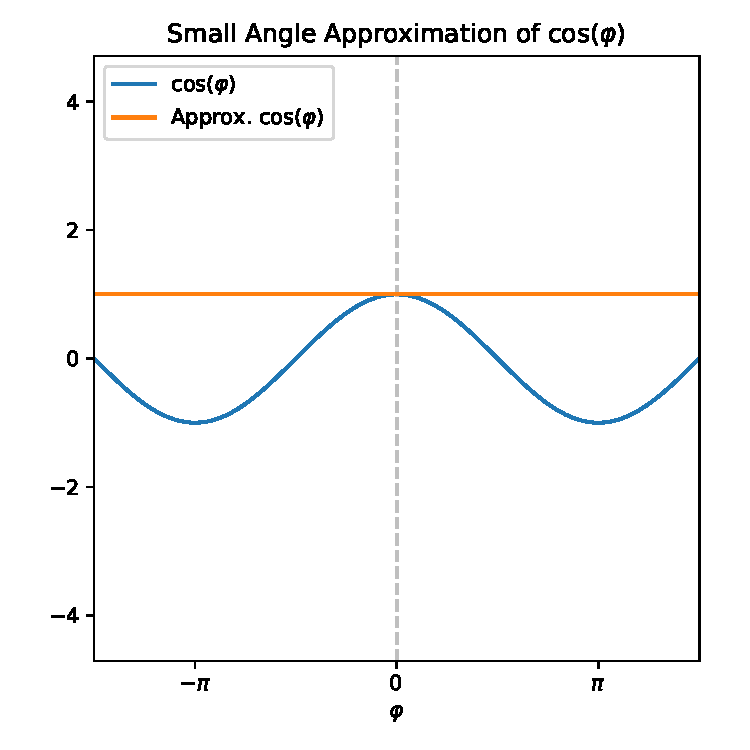
\includegraphics[width = \linewidth]{figures/introduction/generated/small-angle-approximation-cos.pdf}
			\caption{Small angle approximation \( \cos(\varphi) \approx 1 \) of Cosine.}
		\end{subfigure}
		\caption{Visualization of the small angle approximation (given in orange) of the basic trigonometric functions Sine and Cosine (given in blue). It is clear that the approximation is only valid in a small region around zero (\( \varphi \approx 0 \)).}
		\label{fig:smallAngleApproximation}
	\end{figure}

	We now look at two examples of dynamical systems, one of which is linear and one that is not.

	\paragraph{Harmonic Oscillator}
		\label{subsec:harmonicOscillator}

		\begin{figure}
			\centering
			\tikzHarmonicOscillator
			\caption{Illustration of a simple harmonic oscillator with mass \(m\), spring stiffness \(k\) and position \(x\) that is not affected by any external force like gravity. The mass is in equilibrium if \( x = 0 \).}
			\label{fig:simpleHarmonicOscillator}
		\end{figure}

		The \emph{simple harmonic oscillator} describes the dynamical system of a mass \(m\) that is attached to a spring that is following Hooke's Law with stiffness \(k\) (see~\autoref{fig:simpleHarmonicOscillator}). This harmonic oscillator is described by the \ac{ode}
		\begin{equation}
			m\ddot{x} = -kx \quad\iff\quad \ddot{x} = -\frac{k}{m} x  \label{eq:harmonicOscillator}
		\end{equation}
		where \(x\) and \(\ddot{x}\) are the position and acceleration of the mass, respectively. Note that if \( x = 0 \), the mass is in equilibrium and no force is acting on it.

		By using basic results in the solution theory of linear \acp{ode}, we see that the general solution is given as
		\begin{equation*}
			x(t) = A \cos\Big(t \sqrt{k / m} + \varphi\Big)
		\end{equation*}
		with the amplitude \(A\) and the phase \(\varphi\) (see~\autoref{app:harmonicOscillatorSolution} for the derivation of the solution). As neither gravity nor damping or other external forces are involved in the dynamical system, the motion continues forever with a non-changing amplitude.
	% end

	\paragraph{Simple Pendulum}
		\label{subsec:simplePendulum}

		\begin{figure}
			\centering
			\tikzSimplePendulum
			\caption{Illustration of an inverse pendulum with mass \(m\) and displacement \(\varphi\) that is only affected by gravity and no other external force. The mass is in equilibrium for both \( \varphi = 0 \) and \( \varphi = \pi \), where the former is an unstable equilibrium.}
			\label{fig:simplePendulum}
		\end{figure}

		The \emph{inverse pendulum} describes the dynamical system of a mass \(m\) that is attached to a rigid pole of length \(L\) which can freely swing around a suspension point (see~\autoref{fig:simplePendulum}). The pendulum stands upright if \( \varphi = 0 \) and its equation of motion is described by the \ac{ode}
		\begin{equation*}
			\ddot{\varphi} = \frac{g}{L} \sin(\varphi)
		\end{equation*}
		where \(g\), \(L\), \(\varphi\) and \(\ddot{\varphi}\) describe the gravity acceleration, pole length, displacement and acceleration of the mass, respectively. Note that if \( \varphi = 0 \), the mass is in an unstable equilibrium and no force is acting on it.

		In comparison to the harmonic oscillator (\autoref{subsec:harmonicOscillator}), this differential equation is nonlinear. And, even for the case with unit gravity acceleration \( g = 1 \) and unit pole length \( L = 1\), where the \ac{ode} looks really simple
		\begin{equation}
			\ddot{\varphi} = \sin(\varphi)  \label{eq:inversePendulum}
		\end{equation}
		it is not tractable analytically (\ac{ie} there exists no solution in closed form).

		Still, we can apply the small angle approximation introduced before (in this case, \( \sin(\varphi) \approx \varphi \)) which yields the simple \ac{ode}
		\begin{equation}
			\ddot{\varphi} \approx \varphi  \label{eq:linearizedInversePendulum}
		\end{equation}
		solved by
		\begin{equation*}
			\varphi(t) = \frac{1}{2} e^{-t} \big(\varphi_0 + e^{2t} \varphi_0 - \dot{\varphi}_0 + e^{2t} \dot{\varphi}_0\big)
		\end{equation*}
		where \(\varphi_0\) and \(\dot{\varphi}_0\) are the initial displacement and velocity, respectively.

		However, this small angle approximation can only forecast small displacements \( \varphi \ll \pi/2 \). And, as the equilibrium at \( \varphi = 0 \) is unstable, the approximation becomes worse as time goes by because the pendulum falls down. This behavior is shown in~\autoref{fig:inversePendulumApprox}.

		\begin{figure}
			\centering
			\begin{subfigure}[t]{0.5\linewidth}
				\centering
				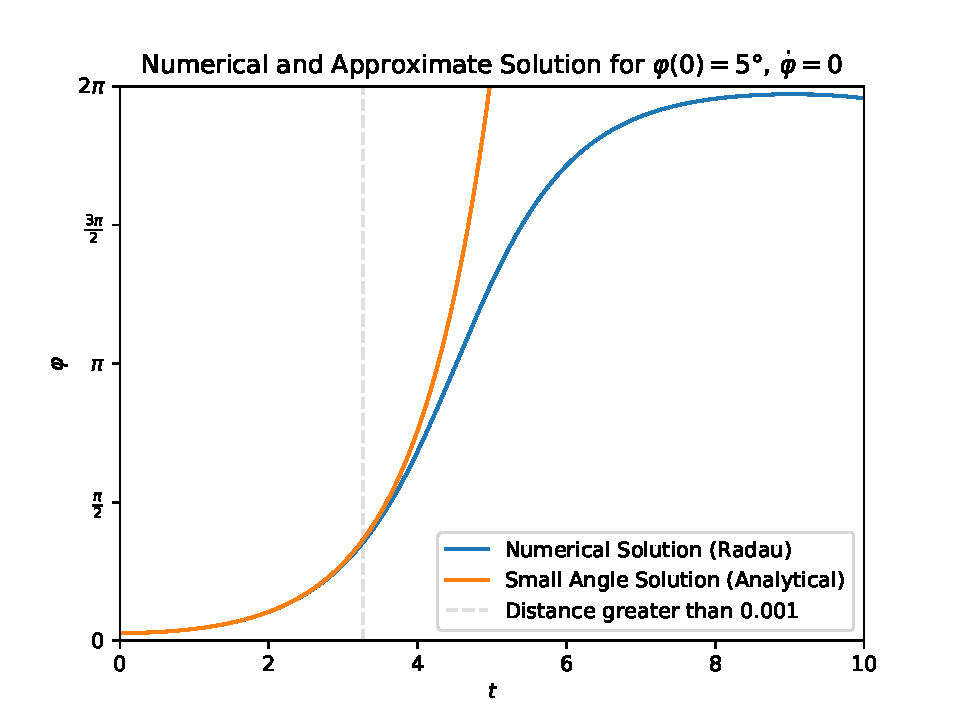
\includegraphics[width = \linewidth]{figures/introduction/generated/pendulum-motion-solutions}
				\caption{Trajectories of two solution strategies to the inverse pendulum, where the blue is a numerical solution of the actual motion of equation (solved using the Radau~IIA method~\cite[72]{hairerSolvingOrdinaryDifferential1996}) and the orange one is the analytically computed solution linearized \ac{ode}. The latter is linearized using small angle approximation. The dashed gray vertical line shows when the distance tolerance of \( \varepsilon = 10^{-3} \) is exceeded.}
			\end{subfigure}%
			~
			\begin{subfigure}[t]{0.5\linewidth}
				\centering
				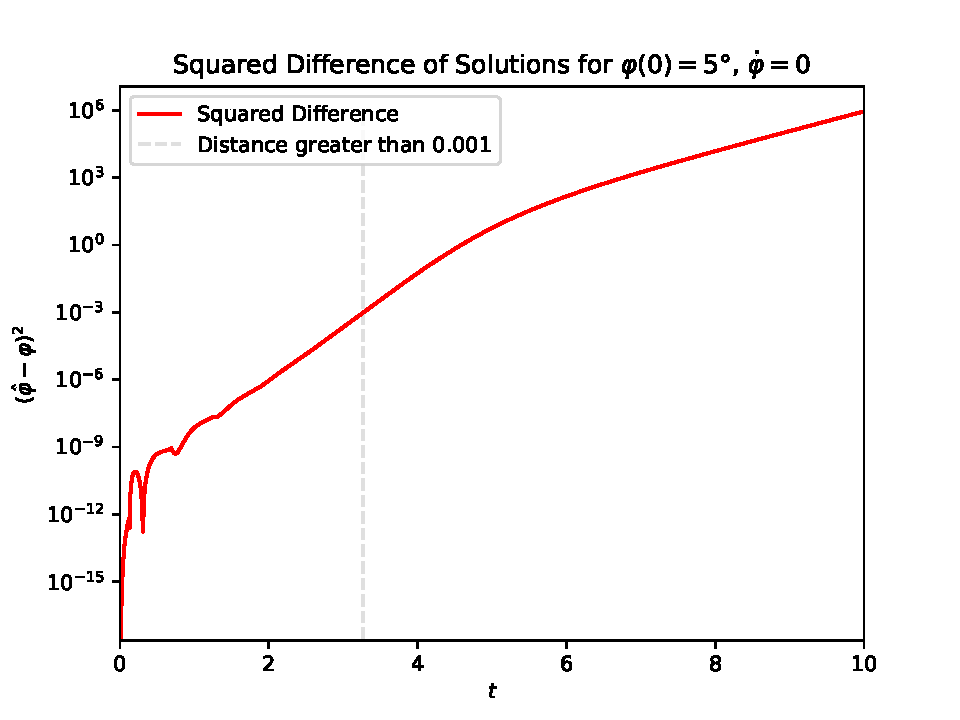
\includegraphics[width = \linewidth]{figures/introduction/generated/pendulum-motion-difference}
				\caption{Differences between the small angle approximation and the numerical solution of the \ac{ode}. The dashed gray vertical line shows when the distance tolerance of \( \varepsilon = 10^{-3} \) is exceeded.}
			\end{subfigure}
			\caption{Comparison of a numerical solution to the \ac{ode} of the inverse pendulum given in\eqref{eq:inversePendulum} and the analytical solution of the linearized \ac{ode} given in\eqref{eq:linearizedInversePendulum}. A tolerance value of \( \varepsilon = 10^{-3} \) is used to show when both solutions diverge from each other.}
			\label{fig:inversePendulumApprox}
		\end{figure}
	% end

	\subsection{Discrete-Time Dynamical Systems}
		In comparison to continuous-time dynamical systems described by \acp{ode}, discrete-time systems are described by a \emph{dynamics function} \( \vec{F} : \R^n \to \R^n \) advancing all states forward in time:
		\begin{equation*}
			\vec{x}_{t + 1} = \vec{F}(\vec{x}_t)
		\end{equation*}
		But we should note that, while seeming more restrictive, discrete-time dynamical systems are more general than continuous-time systems as we can discretize every continuous-time system
		\begin{equation*}
			\dot{\vec{x}} = \vec{f}(\vec{x})
		\end{equation*}
		as a discrete-time dynamical system
		\begin{equation*}
			\vec{x}_{t + 1} = \vec{F}(\vec{x}_t)
		\end{equation*}
		using the state dynamics function
		\begin{equation*}
			\vec{F}\big(\vec{x}(t_0)\big) = \vec{x}(t_0 + \Delta_t) = \vec{x}(t_0) + \int_{t_0}^{t_0 + \Delta_t} \! \vec{f}\big(\vec{x}(\tau)\big) \dd{\tau}
		\end{equation*}
		where \( \Delta_t \) is called the \emph{discretization interval} and \( \vec{x}_k = \vec{x}(k \Delta_t) \). From the Nyquist-Shannon sampling theorem, we know for band-limited functions that the sampling rate \( f_s = 1/\Delta_t \) has to be greater than two times the maximum frequency of the original function~\cite{shannonCommunicationPresenceNoise1949}, \ac{ie} \( f_s = 1/\Delta_t > 2 f \).
	% end
% end
